\chapter{Elméleti háttér és irodalomkutatás}

Ebben a fejezetben kerül bemutatásra minden jelentősebb alapfogalom,  valamint az azokhoz szorosan kapcsolódó technikák és folyamatok, amelyek ismerete nélkülözhetetlen a videó streaming megértéséhez, illetve annak szoftveres megvalósításához.

\section{A videó formátumai}

A videó egy multimédiás eszköz auditív és mozgó vizuális információ tárolására, visszajátszására. Fontos felhasználási területei a bevezetésben is ismertetett média és a szórakoztató ipar.

Egy videó tartalmazhat különböző nyelvű hanganyagokat, mozgóképet, és egyéb metaadatokat -- például feliratokat és miniatűr állóképeket -- mind egy fájlban. Ezek közös tárolására konténerformátumokat alkalmazunk, amelyek megadják, az egyes adatfolyamok hogyan, milyen paraméterekkel, kódolással, tömörítéssel kerüljenek tárolásra, és hogyan kerülhetnek majd lejátszásra.

Szokásos összekeverni, de a konténerformátumoktól függetlenül a mozgóképkódolás és a hangkódolás különálló folyamatok. A kódolás egy algoritmus nyomán az adatot tömöríti, hogy a tárolás és a továbbítás hatékonyabb legyen.

\subsection{Konténerformátumok}

A legelterjedtebb és legszélesebb körben támogatott konténerformátum a Moving Picture Experts Group (MPEG) gondozásában specifikált MP4 -- avagy a sztenderdben használt nevén: MPEG-4 Part 14 --, amely az MPEG-4 projekt részeként született 2001-ben.

Ugyancsak az MPEG gondozásában, az MPEG-2 projekt részeként született 1995-ben az MPEG Transport Stream (MPEG-TS) konténerformátum, amely elsősorban a digitális televíziózásban használatos, és így az internetes videó streaming során is. Felbontja a videóadatokat kisebb, fix hosszú adatcsomagokra, ezzel is előkészítve a tulajdonképpeni kis késleltetésű azonnali továbbítására a videóanyagnak a hálózaton keresztül.

További elterjedt konténerformátumok közé tartozik a Matroska Video (MKV), amely a hibatűréséről ismert; Apple vállalat által macOS-re és iOS-re optimalizálva fejlesztett QuickTime Movie (MOV) formátuma; valamint a WebM, egy szabad felhasználású webes kiszolgálásra optimalizálódott formátum, amelyet nagyobb jelentőségű webböngészők mind támogatnak. Régebbi, már kevésbé használt vagy kivezetett formátumok közé tartozik az Audio Video Interleave (AVI) és a Flash Video (FLV).

\subsection{Mozgókép kódolási módszerei}

Az MPEG-4 projekt keretében született az Advanced Video Coding (AVC) -- avagy H.264 -- kódolási szabvány mozgókép kódolására, amely 2004-ban vált elérhetővé. Továbbra is ez az egyik legelterjedtebb szabvány, a videó streamingben használt konténerformátumok is ezt a kódolást alkalmazzák.

Természetesen azóta több új szabvány is megjelent hasonlóan az MPEG projektjei alatt, mint például az 2013-ban megjelent High Efficiency Video Coding (HEVC) -- avagy H.265 --, amely az AVC-től jobb tömörítést és jobb minőséget ígér, de a licencdíjak miatt nem vált annyira elterjedtté, mint az elődje.

Ezen modern problémák kiküszöbölésére terjedt el a VP8 és a VP9 -- a WebM formátumnak tagjaként --, illetve az AV1 szabad felhasználású kódolási szabványok.

A szabványok konkrét megvalósításával (kodekek) nem foglalkozunk részletesebben, de egy szabad felhasználású és nyílt forráskódú megvalósítása a H.264-nek a x264, amelyet például az FFMpeg szoftvercsomag is használ videó kódolására és dekódolására.

\subsection{Hang kódolási módszerei}

Hanganyag kódolására is több szabványt tudunk megvizsgálni. Ilyen az MPEG Audio Layer III -- rövid nevén: MP3 -- 1991-ből, ezt 1997-ben az Advanced Audio Coding (AAC) szabvány váltotta le. Ezen szabványok az MPEG által kerültek kifejlesztésre, valamint mindkettő veszteséges tömörítést alkalmaz, azaz a kódoláson és dekódoláson átesett hanganyag minősége nem lesz azonos az eredeti hanganyaggal.

Főleg a mozivilágban használt kódolás a Dolby AC-3  -- ismertebb nevén: Dolby Digital. Azonos bitrátánál is az előbbieknél jobb minőséget ígér. 2017-ben már lejárt a szabadalmi védelme, így azóta szabadon felhasználható. Egy másik, születése (2012) óta szabad felhasználású kódolás az Opus, amelyet a Skype és a Discord is használ VoIP alapú kommunikációra, és az összes eddig említett kódolásnál jobb minőséget produkál.

Természetesen találkozhattunk tömörítetlen (pl.: WAV), illetve veszteségmentes kódolásokkal is (pl.: FLAC) is, azonban a streaming világában ezek nem használatosak, mivel a nagyobb fájlméretük meghaladná a sávszélesség és a tárhely korlátait. Az AC-3 és AAC szabványok közül szokás választani a videó streaming során, széles körben kompatibilisek mindenféle lejátszó eszközzel, míg az Opus még nem eléggé támogatott.

\section{Videó streaming kiszolgálása}

A médiastreamelés egy olyan folyamat, amely során az médiaadatokat -- mi esetünkben videóadatot -- egy adott hálózati protokoll felett, egy adott konténerformátumban, adott kódolásssal továbbítjuk a végfelhasználók számára. Elsősorban az azonnali elérhetőségre összpontosít, azaz a lejátszásnak a lehető legkisebb késleltetéssel kell megtörténnie, kevésbé fontos a streaming során a minőség megtartása, mint ahogy az fontos lenne teljes médiumok egyben való letöltésekor.

A streaming során az adatfolyamba helyezés előtt a videóadatokat újrakódoljuk, majd kisebb adatcsomagokra -- úgynevezett ``packetekre'' -- bontjuk, és ezeket a csomagokat a hálózaton keresztül továbbítjuk a végfelhasználók felé. Az adatcsomagok önmagukban is értelmezhetőek, és a végfelhasználók lejátszó alkalmazásai képesek az adatcsomagokat a megfelelő sorrendben és időzítéssel lejátszani. A streaming könnyen reagál a lejátszás során ugrálásokra, előre- és visszatekerésre, mivel a videót nem kell teljes egészében letölteni a végfelhasználói eszközre, hanem a feldarabolt videócsomagot a lejátszás során továbbítjuk abban a pillanatban, amikor arra szükség lesz.

\subsection{Az élő közvetítés és video-on-demand különbségei}

Annak megfelelően, hogy az adat egésze mikor áll rendelkezésünkre, kettő fő streaming típust különböztetünk meg: az élő közvetítést (live streaming) és a video-on-demand (VOD) streaminget. A VOD esetében a videóadatokat előre rögzített formában tároljuk, és a végfelhasználók a videóadatokat a saját időbeosztásuknak megfelelően nézhetik meg. Az élő közvetítés esetében a videóadatokat valós időben továbbítjuk a végfelhasználók felé, és a végfelhasználók a videóadatokat a közvetítés során nézhetik meg.

Különbözik mindkettőnél, hogy milyen fizikai infrastrukturális tervezést kell végrehajtani a legjobb kiszolgálás érdekében. Élő adásoknál a késleltetés a középponti kihívás, mivel a videóadatokat a lehető leggyorsabban kell továbbítani a végfelhasználók felé, hogy a közvetítés valóban élőnek tűnjön, ehhez magas számítási teljesítmény szükséges. A VOD esetében a hálózati sávszélességből adódó problémák leküzdése a központi kihívás, mivel a videót a felhasználók sokkal nagyobb közönsége kívánja elérni, azt kiváló minőségben szeretné megtekinteni, ennek ellenére a globális sávszélesség korlátozott. Itt a caching és a tartalomterjesztés optimalizálása a kulcs, ekkor jönnek képbe a Content Delivery Networkök (CDN-ek), azaz a tartalomterjesztő hálózatok.

Üzleti szempontból a bevétel az élő adások során a közbeiktatott reklámokból származik főleg és a pay-per-view rendszerekből, míg a VOD esetében a közbeiktatott reklámokon kívül a felhasználók előfizetési díjából, tranzakcionális egyszeri vásárlásból -- amennyiben a reklámokat kerülni szeretnék.

\subsection{Adaptive Bitrate Streaming}

A streamelést erősen befolyásoló tényező a hálózati feltételek változása, amelyek a videólejátszás minőségét és késleltetését is befolyásolják. Az Adaptive Bitrate Streaming (ABR) egy a hálózati kiszolgálás során alkalmazott technika, amely megoldást jelenthet erre a problémára.

Az ABR során a forrásvideót több különböző bitrátával dolgozó kodekekkel és különböző felbontással kódoljuk a médiaszerveren, majd lejátszáskor a lejátszó alkalmazás a hálózati feltételek változására reagálva, valamint a fogadó fél számítási kapacitásától függően valós időben választja ki a megfelelő vi\-de\-ó\-strea\-met ezek közül, onnan válogatja a packeteket (\refstruc{fig:ABR}).

\begin{figure}[ht]
	\centering
	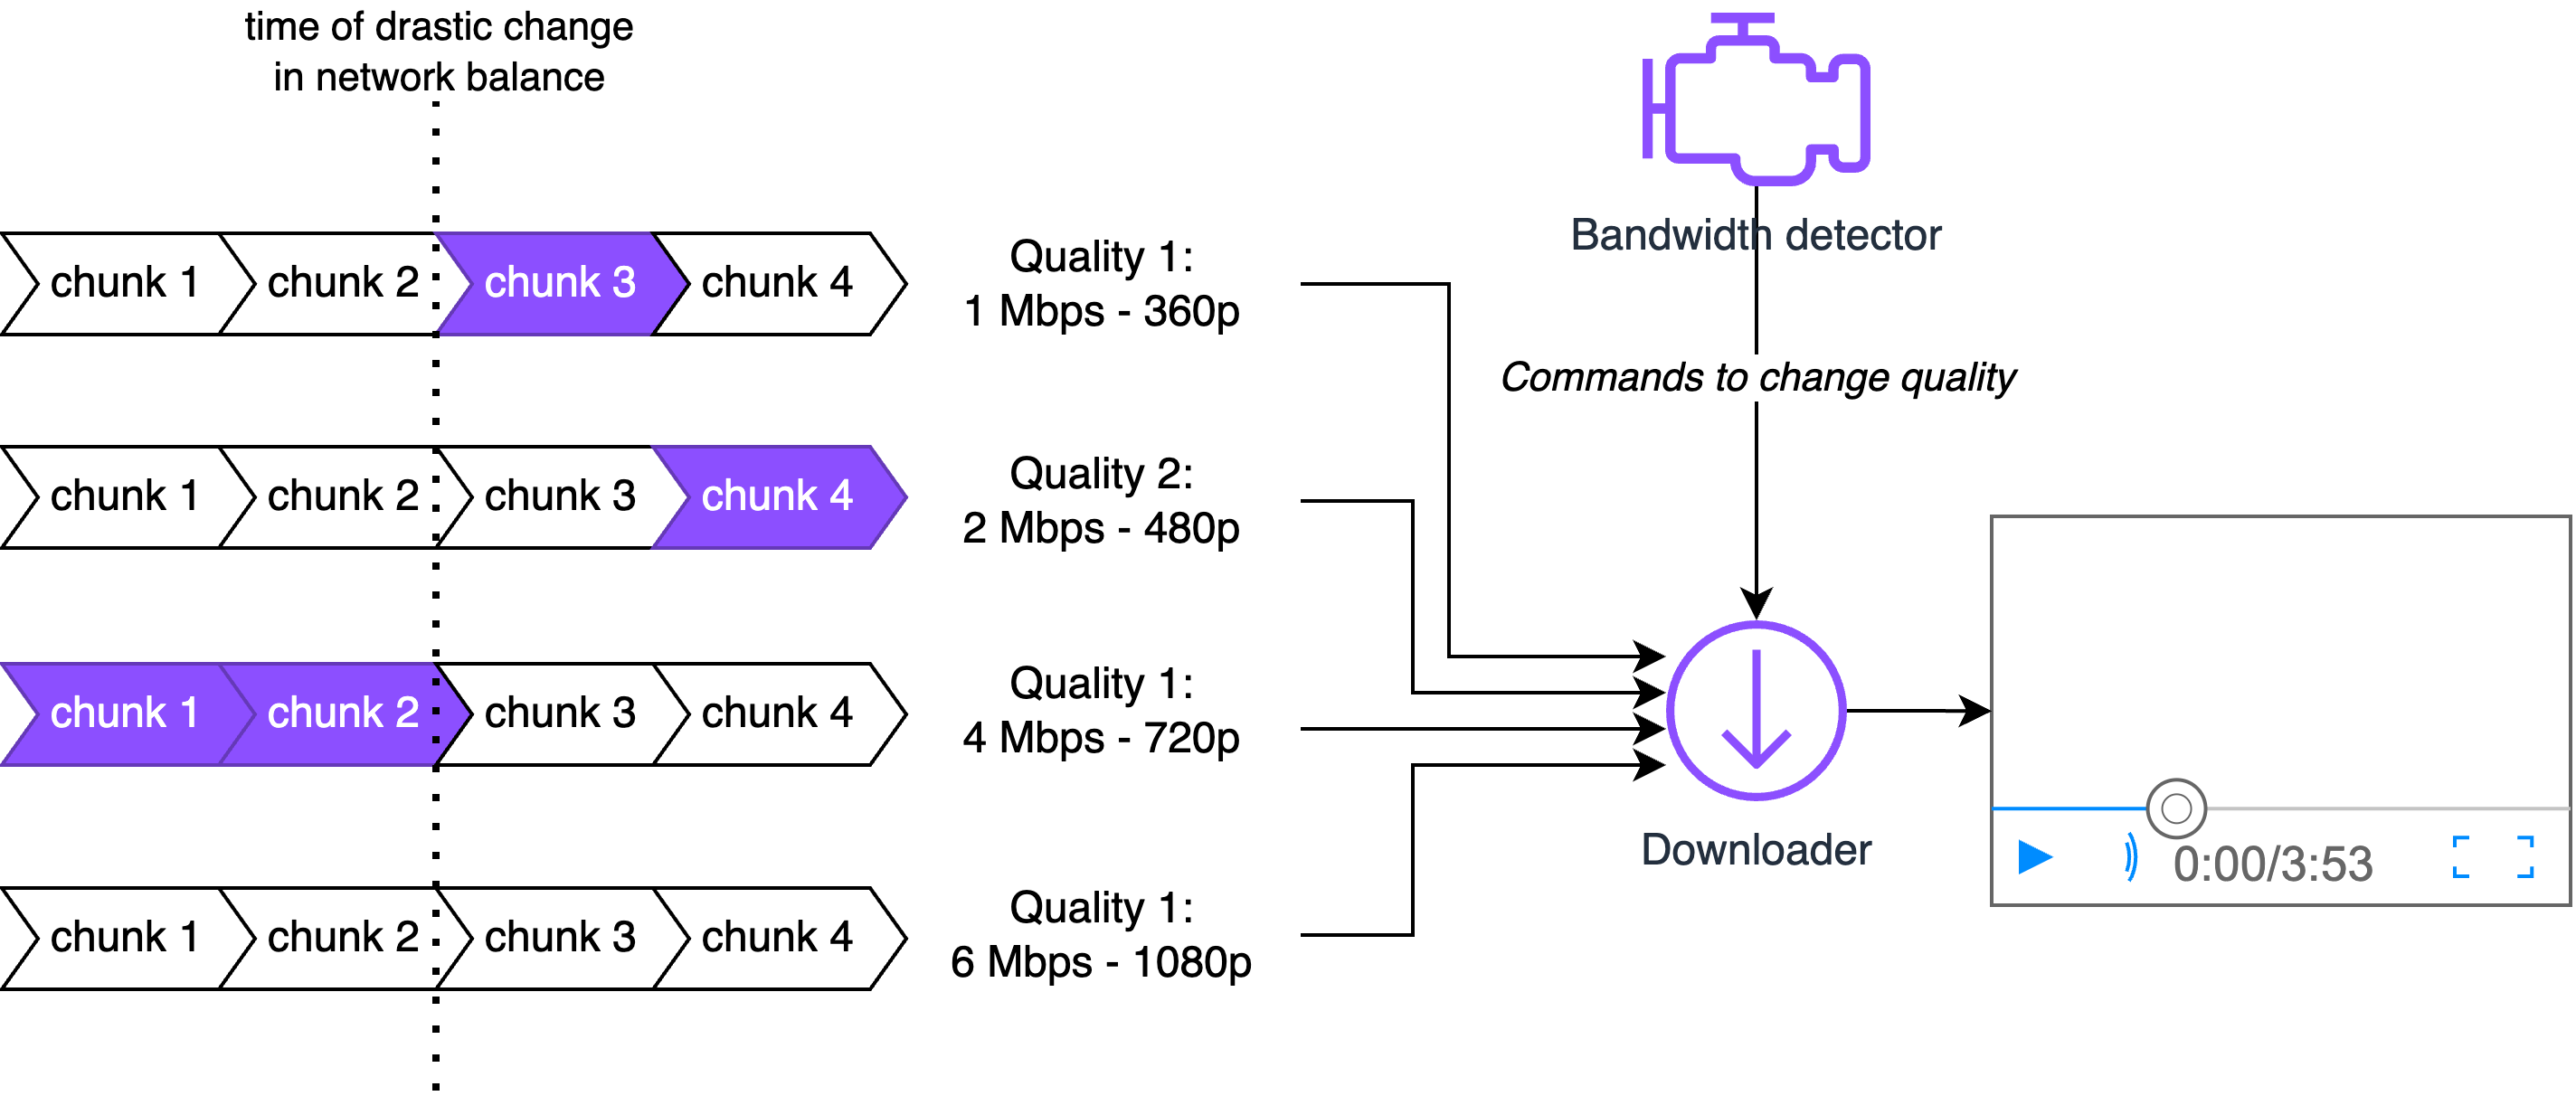
\includegraphics[width=140mm, keepaspectratio]{figures/dipterv_abr.png}
	\caption{Az Adaptive Bitrate Streaming működése.}
	\label{fig:ABR}
\end{figure}

\section{Videó streaming hálózati protokolljai}

Videó streamelésére -- másképp fogalmazva: valamely korábban ismertetett formátumban tárolt videó adatfolyamba való illesztésére különböző hálózati protokollok palettája áll rendelkezésünkre.

Ez a szekció az alkalmazás rétegben alkalmazott protokollok (Layer 7) közül vizsgál meg néhány streaming használatára elterjedt protokollt, megemlítve, milyen szállítási rétegű protokollokkal (Layer 4) tudnak együttműködni.

\subsection{Real-Time Messaging Protocol}

TODO

\subsection{HTTP Live Streaming}

TODO

\subsection{Dynamic Adaptive Streaming over HTTP}

TODO

\subsection{WebRTC}

A források és a streamet figyelők számának kardinalitása szempontjából ez a protokoll a legjobb választás, amennyiben a felhasználási célja az, hogy a felhasználók közvetlenül egymással kommunikálhassanak, és nem szükséges közbeiktatni egy központi médiaszervert. 

TODO: még egy keveset ide, hogy lássa az olvasó később, hogy miért nem lesz releváns a mi választásunkban az implementáció során.
